% generated by experiments/make_tex_figures.py -- do not edit by hand
\begin{figure}[t]
\centering
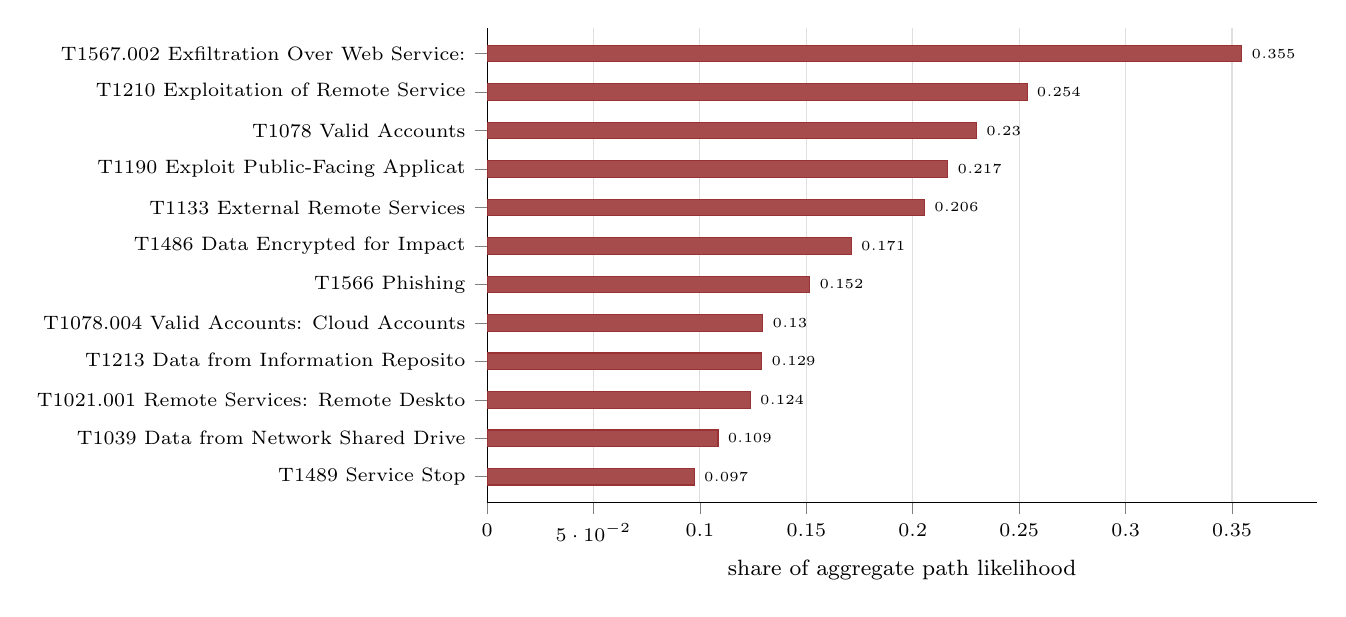
\begin{tikzpicture}
\begin{axis}[
    xbar, width=\linewidth, height=7.6cm,
    xlabel={share of aggregate path likelihood},
    xmin=0, enlarge y limits=0.06,
    ytick={0,1,2,3,4,5,6,7,8,9,10,11}, yticklabels={{T1567.002 Exfiltration Over Web Service:},{T1210 Exploitation of Remote Service},{T1078 Valid Accounts},{T1190 Exploit Public-Facing Applicat},{T1133 External Remote Services},{T1486 Data Encrypted for Impact},{T1566 Phishing},{T1078.004 Valid Accounts: Cloud Accounts},{T1213 Data from Information Reposito},{T1021.001 Remote Services: Remote Deskto},{T1039 Data from Network Shared Drive},{T1489 Service Stop}},
    y dir=reverse, ticklabel style={font=\scriptsize},
    label style={font=\footnotesize},
    nodes near coords, nodes near coords style={font=\tiny},
    every node near coord/.append style={/pgf/number format/fixed,
        /pgf/number format/precision=3},
    xmajorgrids, grid style={gray!25}, axis lines*=left,
    bar width=6pt, tick align=outside,
]
\addplot[fill=Maroon!70, draw=Maroon!80] coordinates {
        (0.354600,0)
        (0.253700,1)
        (0.230000,2)
        (0.216500,3)
        (0.205600,4)
        (0.171200,5)
        (0.151600,6)
        (0.129600,7)
        (0.129100,8)
        (0.123700,9)
        (0.108500,10)
        (0.097400,11)
};
\end{axis}
\end{tikzpicture}
\caption{MITRE ATT\&CK techniques ranked by the share of aggregate path likelihood that traverses them (Enterprise and ICS matrices combined).}
\label{fig:techniques}
\end{figure}
